\chapter{Modelo Entidad-Relación}

\section{Reglas semánticas}

A continuación se describen las 12 entidades que conforman el modelo, detallando los atributos que las caracterizan y las restricciones semánticas que las gobiernan. Las entidades se agrupan por módulo funcional para facilitar su comprensión.

\vspace{0.5cm}
\noindent \textbf{Módulo 1: Organización y Misión}

\begin{itemize}
    \item \textbf{Agencia} es la entidad que representa a la corporación, gobierno u organismo propietario de los activos espaciales. Toda agencia es identificada de forma única por un \texttt{ID\_Agencia} surrogado. Posee un \texttt{Nombre} obligatorio y único, un \texttt{Pais} sede, un \texttt{Tipo} que discrimina si es organización privada o gubernamental, el \texttt{Año\_Fundacion} y un \texttt{Sitio\_Web} de referencia.
    \item \textbf{Constelacion} agrupa al conjunto de satélites que comparten una misión común bajo la responsabilidad de una \texttt{Agencia}. Posee un \texttt{Nombre\_Mision} obligatorio, un \texttt{Proposito} descriptivo y una \texttt{Fecha\_Inicio} de operaciones.
    \item \textbf{Operador} representa al personal técnico de SpaceTech habilitado para interactuar con el sistema. Posee un \texttt{Nombre}, un \texttt{Correo} corporativo único, un atributo \texttt{Rol} que discrimina su función (Administrador, Ingeniero de Vuelo, Operador de Estación, Analista de Seguridad) y una \texttt{Fecha\_Contratacion}. Es la entidad que registra la responsabilidad humana sobre cada acción operativa del sistema.
\end{itemize}

\vspace{0.5cm}
\noindent \textbf{Módulo 2: Objetos Espaciales (Jerarquía de Herencia)}

\begin{itemize}
    \item \textbf{Objeto\_Espacial} es la superclase abstracta que unifica todo objeto rastreado en órbita, independientemente de si es un activo operativo o un fragmento de basura. Registra el \texttt{NORAD\_ID} (identificador internacional del catálogo de objetos espaciales, clave única alternativa), la \texttt{Altitud\_Actual\_km} y la \texttt{Velocidad\_km\_s} reportadas por los sistemas de rastreo, y un atributo discriminador \texttt{Tipo\_Objeto} que determina si el registro pertenece a la subclase \texttt{Satelite} o \texttt{Basura\_Espacial}. Esta entidad implementa el patrón Table Per Subclass (JOINED).
    \item \textbf{Satelite} es la subclase de \texttt{Objeto\_Espacial} que representa los activos operativos de SpaceTech. Extiende la superclase con los atributos específicos del activo: \texttt{ID\_Constelacion} (FK), \texttt{ID\_Orbita} (FK), \texttt{Estado} operativo (Activo, Mantenimiento, Destruido), \texttt{Masa\_kg}, \texttt{Fecha\_Lanzamiento} y \texttt{Vida\_Util\_Años}. La participación es total: todo satélite debe existir primero como \texttt{Objeto\_Espacial}.
    \item \textbf{Basura\_Espacial} es la subclase de \texttt{Objeto\_Espacial} que representa los fragmentos inertes rastreados por radar. Extiende la superclase con \texttt{Descripcion\_Origen} (misión que lo generó), \texttt{Tamaño\_mts} estimado, \texttt{Nivel\_Riesgo} y \texttt{Fuente\_Radar} (agencia que proveyó los datos del objeto).
    \item \textbf{Orbita} es la entidad catálogo que define los parámetros de la trayectoria objetivo de un satélite. Registra el \texttt{Tipo\_Orbita} (LEO, MEO, GEO, SSO), el \texttt{Apogeo\_km}, el \texttt{Perigeo\_km}, la \texttt{Inclinacion\_grados} y el \texttt{Periodo\_min} de la órbita. Se modela como entidad independiente para que múltiples satélites de la misma constelación puedan referenciar la misma definición orbital sin redundancia.
\end{itemize}

\vspace{0.5cm}
\noindent \textbf{Módulo 3: Operaciones Terrestres}

\begin{itemize}
    \item \textbf{Estacion\_Terrena} representa las instalaciones físicas en tierra equipadas con antenas para comunicarse con los satélites. Registra \texttt{Nombre\_Instalacion}, \texttt{Pais}, coordenadas geográficas (\texttt{Latitud}, \texttt{Longitud}) y el \texttt{Diametro\_Antena\_m} de la antena principal. Toda estación está asignada a un \texttt{Operador} responsable (FK), lo que conecta esta entidad al módulo de personal.
    \item \textbf{Contacto\_Estacion} es la entidad transaccional que registra cada ventana de comunicación establecida entre un \texttt{Satelite} y una \texttt{Estacion\_Terrena}. Resuelve la relación N:M natural entre ambas entidades. Registra el \texttt{Timestamp\_Inicio}, el \texttt{Timestamp\_Fin} (nullable durante la sesión activa), la \texttt{Calidad\_Senal\_dB} y el \texttt{Volumen\_Datos\_MB} transferido.
\end{itemize}

\vspace{0.5cm}
\noindent \textbf{Módulo 4: Monitoreo de Salud (Alta Transaccionalidad)}

\begin{itemize}
    \item \textbf{Telemetria} es la entidad de mayor volumen del sistema. Registra los signos vitales de cada satélite en un instante de tiempo determinado: \texttt{Timestamp\_Lectura}, \texttt{Temperatura\_C}, \texttt{Bateria\_Pct}, \texttt{Voltaje\_V}, \texttt{Altitud\_Real\_km}, \texttt{Posicion\_Latitud} y \texttt{Posicion\_Longitud}. Utiliza \texttt{BIGINT} como PK surrogada dado el volumen esperado de millones de registros diarios.
\end{itemize}

\vspace{0.5cm}
\noindent \textbf{Módulo 5: Seguridad Orbital}

\begin{itemize}
    \item \textbf{Evento\_Colision} registra la alerta formal generada cuando los sistemas de vigilancia detectan una probabilidad de colisión entre un satélite activo y un objeto de basura espacial. Vincula a un \texttt{Satelite} (FK) con una \texttt{Basura\_Espacial} (FK) en un instante específico, registrando el \texttt{Timestamp\_Estimado} de máxima aproximación, la \texttt{Probabilidad\_Choque} calculada, la \texttt{Distancia\_Min\_km} predicha y el \texttt{Estado\_Alerta} actual (Emitida, Maniobra Autorizada, Esquivada, Falsa Alarma).
    \item \textbf{Maniobra\_Evasiva} registra la respuesta operativa ejecutada ante un \texttt{Evento\_Colision}. Es la entidad que cierra el ciclo de trazabilidad del sistema: vincula el evento de riesgo con el \texttt{Operador} que autorizó la respuesta y documenta el \texttt{Tipo\_Maniobra} (Alzamiento Orbital, Descenso Orbital, Ajuste Lateral), el \texttt{Delta\_V\_ms} aplicado (cantidad de variación de velocidad), el \texttt{Timestamp\_Ejecucion} y el \texttt{Resultado} obtenido (Exitosa, Fallida, Cancelada).
\end{itemize}

\section{Modelo Entidad-Relación}

La figura 2.1 presenta el diagrama Entidad-Relación del sistema de base de datos de SpaceTech, modelado bajo la notación de Pata de Gallo (Crow's Foot). El diagrama refleja la estructura completa de las 12 entidades descritas en la sección anterior, sus atributos, llaves primarias, llaves foráneas, cardinalidades y la jerarquía de herencia implementada para \texttt{Objeto\_Espacial}.

\begin{figure}[H]
	\centering
	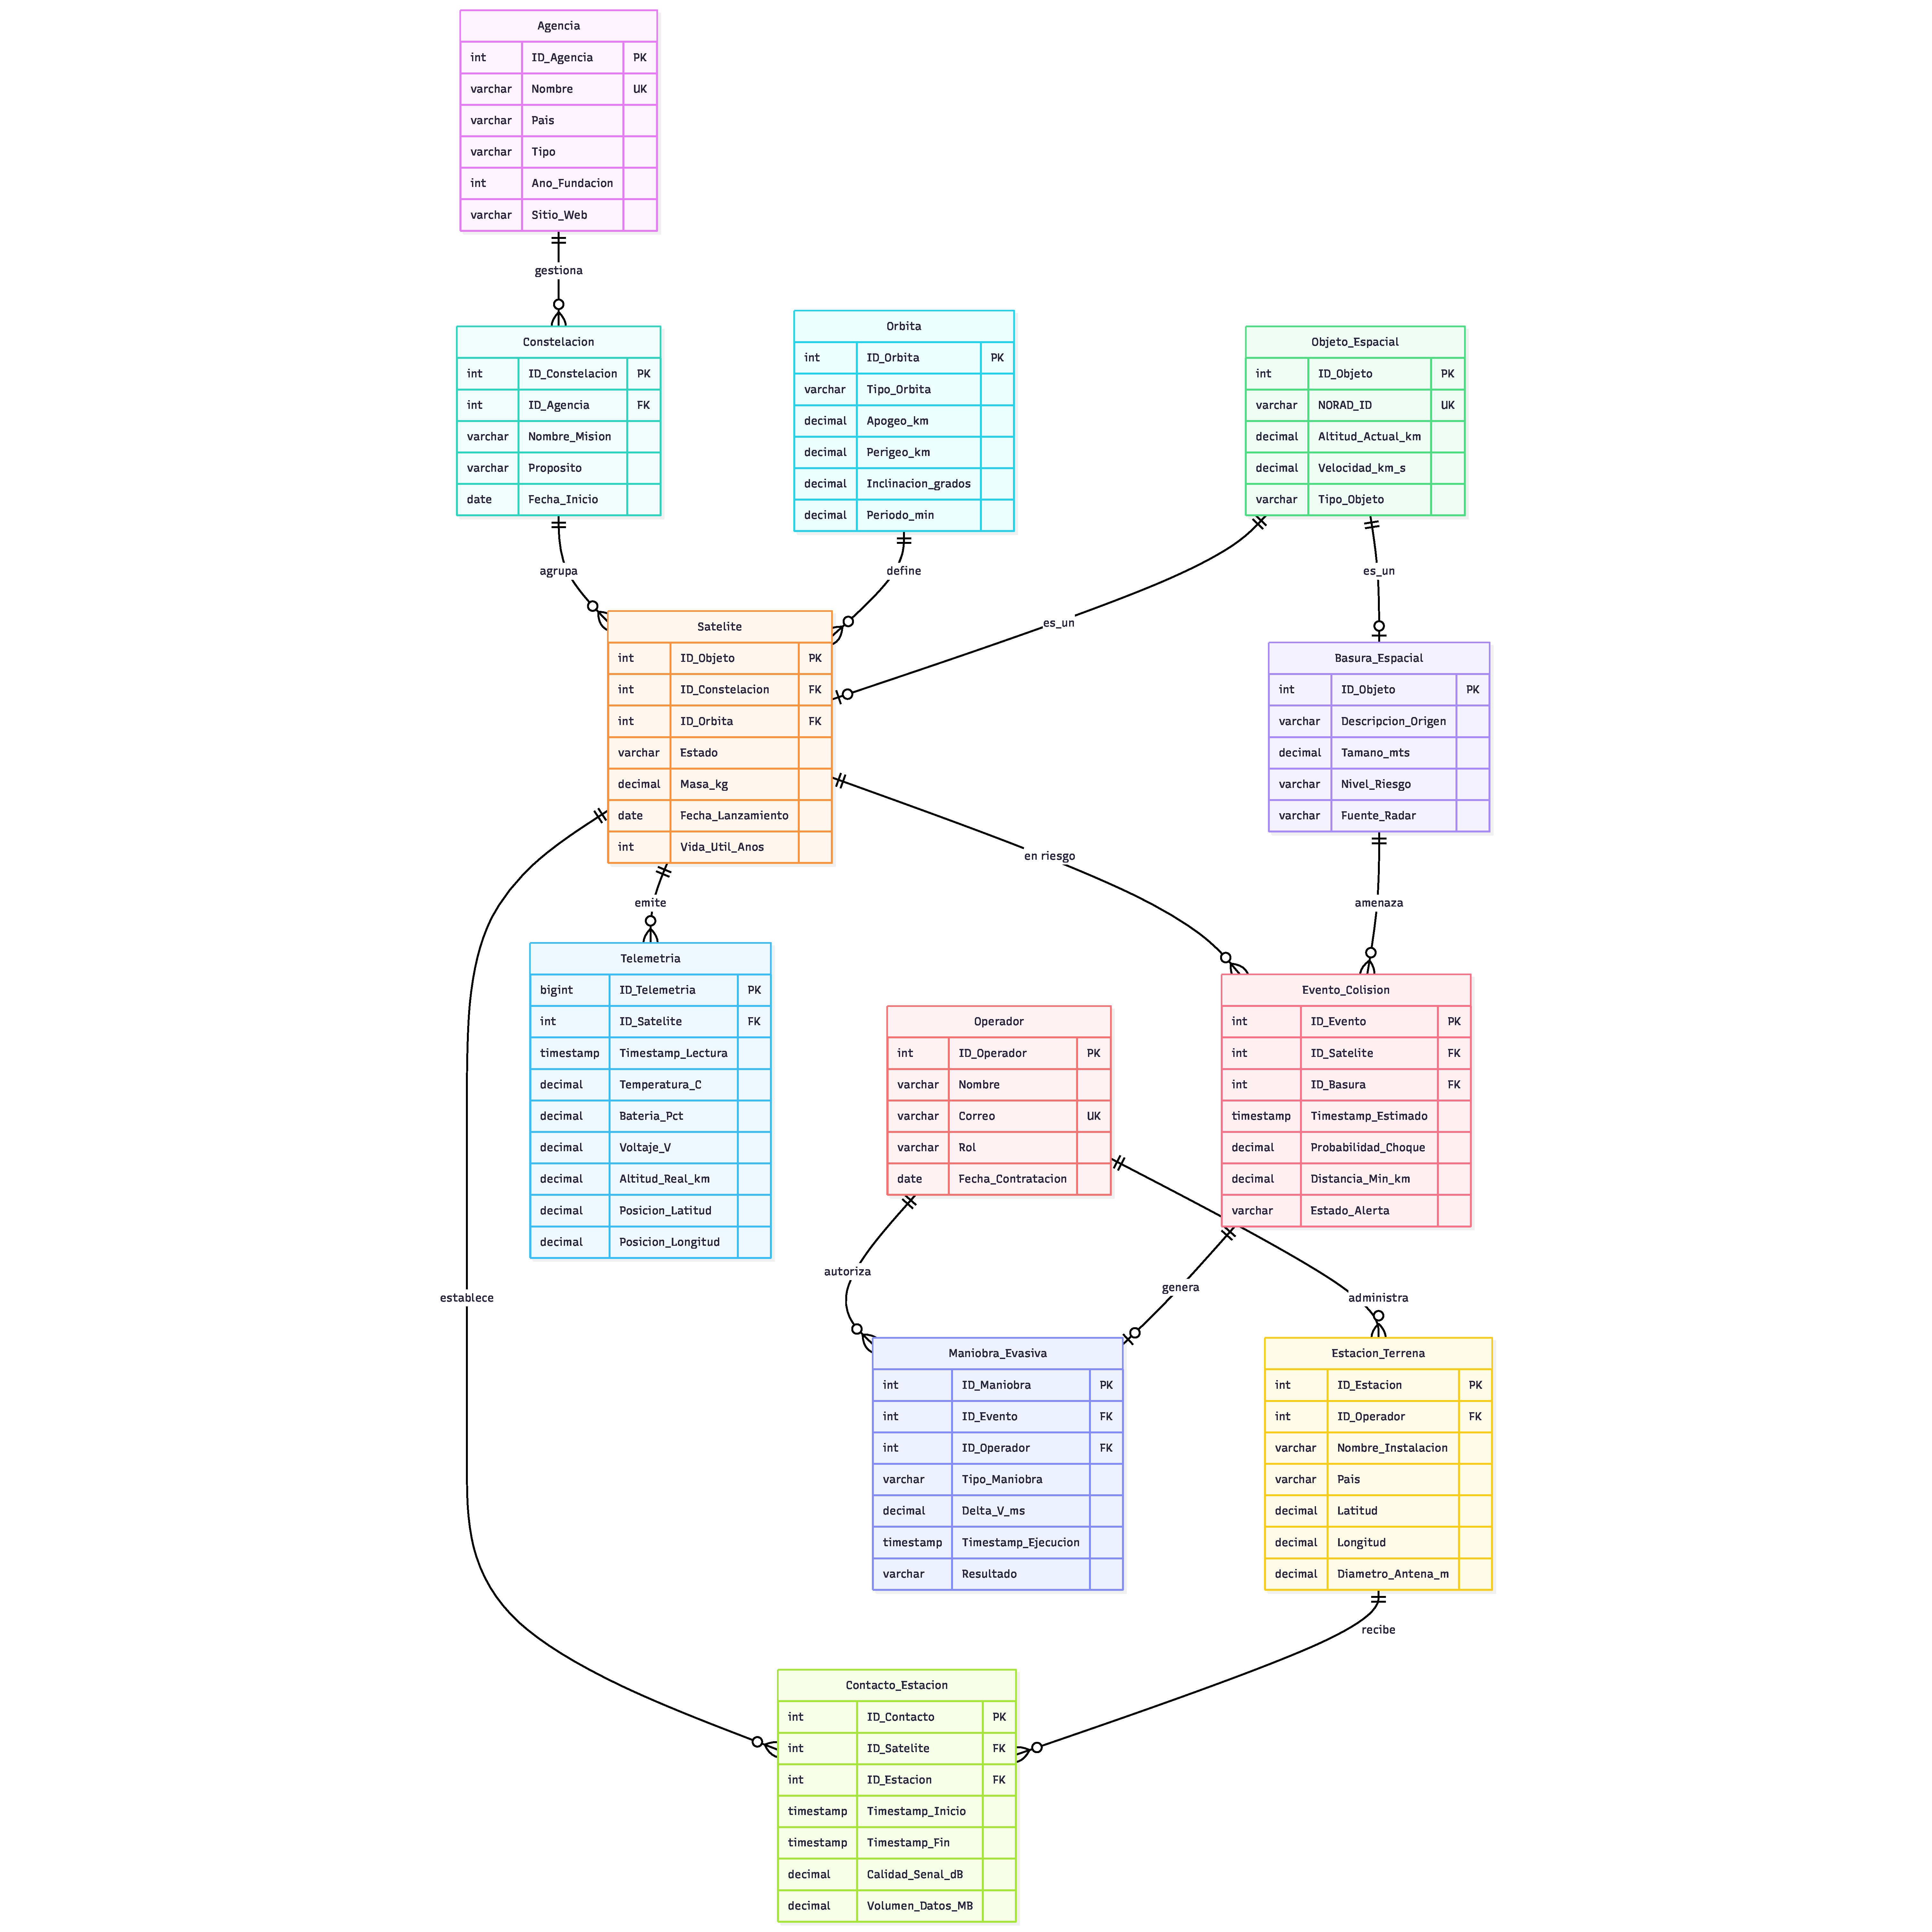
\includegraphics[width=\textwidth,height=0.82\textheight,keepaspectratio]{Diagrama.pdf}
	\caption{Diagrama Entidad-Relación SpaceTech (Notación Pata de Gallo)}
\end{figure}

\section{Especificaciones y consideraciones sobre el modelo}

A continuación se detalla, entidad por entidad, las especificaciones funcionales y las decisiones de diseño que justifican su estructura dentro del modelo relacional.

\subsection{Agencia}

\begin{itemize}
    \item \textbf{Especificaciones:} Almacena los datos corporativos de cada organización propietaria: \texttt{ID\_Agencia} (PK surrogada), \texttt{Nombre} (UK), \texttt{Pais}, \texttt{Tipo}, \texttt{Año\_Fundacion} y \texttt{Sitio\_Web}.
    \item \textbf{Consideraciones:} La PK seleccionada es \texttt{ID\_Agencia}, una clave surrogada autoincremenal, en lugar del nombre de la agencia. Si bien el nombre identifica unívocamente a una organización, es un dato de negocio sujeto a cambios (fusiones, rebrandings); actúa como clave única alternativa (UK). Catálogo de gestión exclusiva del Administrador de Misiones.
\end{itemize}

\subsection{Constelacion}

\begin{itemize}
    \item \textbf{Especificaciones:} Almacena la agrupación de satélites por misión: \texttt{ID\_Constelacion} (PK), \texttt{ID\_Agencia} (FK, NOT NULL), \texttt{Nombre\_Mision} (NOT NULL), \texttt{Proposito} y \texttt{Fecha\_Inicio}.
    \item \textbf{Consideraciones:} La FK \texttt{ID\_Agencia} es NOT NULL: toda constelación debe pertenecer a una agencia conocida (participación total). La relación con \texttt{Agencia} es N:1 desde Constelacion: una agencia puede gestionar múltiples misiones.
\end{itemize}

\subsection{Operador}

\begin{itemize}
    \item \textbf{Especificaciones:} Almacena el perfil del personal técnico: \texttt{ID\_Operador} (PK), \texttt{Nombre} (NOT NULL), \texttt{Correo} (UK, NOT NULL), \texttt{Rol} (NOT NULL) y \texttt{Fecha\_Contratacion}.
    \item \textbf{Consideraciones:} \texttt{Correo} actúa como clave única alternativa para el inicio de sesión corporativo. El atributo \texttt{Rol} acepta valores controlados mediante CHECK constraint: Administrador, Ingeniero\_Vuelo, Operador\_Estacion, Analista\_Seguridad. Esta entidad se conecta al sistema operativo en dos puntos: (1) como responsable de una \texttt{Estacion\_Terrena} (1:N) y (2) como autorizante de una \texttt{Maniobra\_Evasiva} (1:N), lo que garantiza la trazabilidad de toda acción operativa.
\end{itemize}

\subsection{Objeto\_Espacial}

\begin{itemize}
    \item \textbf{Especificaciones:} Superclase abstracta del catálogo orbital: \texttt{ID\_Objeto} (PK), \texttt{NORAD\_ID} (UK), \texttt{Altitud\_Actual\_km}, \texttt{Velocidad\_km\_s} y \texttt{Tipo\_Objeto} (discriminador CHECK: Satelite, Basura).
    \item \textbf{Consideraciones:} Esta es la decisión de diseño más importante del módulo orbital: en lugar de tener \texttt{Satelite} y \texttt{Basura\_Espacial} como entidades completamente independientes, se unifica la noción de ``objeto rastreado en órbita'' en una superclase. Esto permite que \texttt{Evento\_Colision} referencie ambos tipos de objeto de forma limpia sin duplicar atributos comunes. El \texttt{NORAD\_ID} (número del catálogo de la Space Surveillance Network) es único mundialmente y actúa como clave alternativa de negocio. Se implementa el patrón Table Per Subclass (JOINED) siguiendo la metodología de Ramakrishnan Cap. 3. \textbf{Nota de implementación:} el patrón JOINED garantiza la herencia estructural, pero no impide en SQL puro que un mismo \texttt{ID\_Objeto} tenga registros simultáneos en \texttt{Satelite} y en \texttt{Basura\_Espacial}. La disjunción se refuerza en dos capas: (1) mediante el atributo discriminador \texttt{Tipo\_Objeto} con restricción CHECK, y (2) mediante un trigger BEFORE INSERT sobre cada subclase que verifica que el \texttt{Tipo\_Objeto} del padre coincide con la subclase que se está insertando, abortando la operación en caso contrario. Esta doble validación garantiza la integridad de la jerarquía a nivel de base de datos sin depender de la capa de aplicación.
\end{itemize}

\subsection{Satelite}

\begin{itemize}
    \item \textbf{Especificaciones:} Subclase de \texttt{Objeto\_Espacial}. Su PK es \texttt{ID\_Objeto} (FK $\rightarrow$ Objeto\_Espacial). Añade \texttt{ID\_Constelacion} (FK), \texttt{ID\_Orbita} (FK), \texttt{Estado}, \texttt{Masa\_kg}, \texttt{Fecha\_Lanzamiento} y \texttt{Vida\_Util\_Años}.
    \item \textbf{Consideraciones:} No se genera una nueva clave en la subclase: \texttt{ID\_Objeto} es a la vez PK y FK (patrón JOINED). La cobertura es total y disjunta: todo objeto de tipo Satelite debe tener exactamente un registro en esta tabla. \texttt{Estado} acepta valores controlados (CHECK): Activo, Mantenimiento, Destruido. La relación con \texttt{Constelacion} es N:1 y con \texttt{Orbita} es N:1.
\end{itemize}

\subsection{Basura\_Espacial}

\begin{itemize}
    \item \textbf{Especificaciones:} Subclase de \texttt{Objeto\_Espacial}. Su PK es \texttt{ID\_Objeto} (FK $\rightarrow$ Objeto\_Espacial). Añade \texttt{Descripcion\_Origen} (nullable para fragmentos no identificados), \texttt{Tamaño\_mts} (nullable), \texttt{Nivel\_Riesgo} y \texttt{Fuente\_Radar}.
    \item \textbf{Consideraciones:} Los atributos \texttt{Descripcion\_Origen} y \texttt{Tamaño\_mts} son nullable porque los fragmentos de menos de 10 cm no son rastreables individualmente; su catalogación es provisional. \texttt{Nivel\_Riesgo} acepta valores controlados (CHECK): Bajo, Medio, Alto, Critico. \texttt{Fuente\_Radar} indica la agencia que reportó el objeto (ESA, NASA, 18SDS), dato clave para la auditoría de la fuente de información.
\end{itemize}

\subsection{Orbita}

\begin{itemize}
    \item \textbf{Especificaciones:} Catálogo de parámetros orbitales: \texttt{ID\_Orbita} (PK), \texttt{Tipo\_Orbita} (NOT NULL), \texttt{Apogeo\_km}, \texttt{Perigeo\_km}, \texttt{Inclinacion\_grados} y \texttt{Periodo\_min}.
    \item \textbf{Consideraciones:} Se modela como entidad independiente (no como atributos de \texttt{Satelite}) para evitar redundancia: múltiples satélites de la misma constelación comparten exactamente los mismos parámetros orbitales objetivo. Extraerlos a una tabla propia cumple la 3FN. \texttt{Tipo\_Orbita} acepta CHECK: LEO, MEO, GEO, SSO, HEO.
\end{itemize}

\subsection{Estacion\_Terrena}

\begin{itemize}
    \item \textbf{Especificaciones:} Registra las instalaciones terrestres: \texttt{ID\_Estacion} (PK), \texttt{ID\_Operador} (FK, NOT NULL), \texttt{Nombre\_Instalacion} (NOT NULL), \texttt{Pais} (NOT NULL), \texttt{Latitud}, \texttt{Longitud} y \texttt{Diametro\_Antena\_m}.
    \item \textbf{Consideraciones:} La FK \texttt{ID\_Operador} conecta cada estación con el operador responsable de su operación, estableciendo una relación 1:N (un operador puede ser responsable de varias estaciones, pero cada estación tiene un único responsable asignado). Esta decisión convierte a \texttt{Operador} en una entidad central del modelo con participación real en el sistema.
\end{itemize}

\subsection{Contacto\_Estacion}

\begin{itemize}
    \item \textbf{Especificaciones:} Registra cada ventana de contacto: \texttt{ID\_Contacto} (PK), \texttt{ID\_Satelite} (FK), \texttt{ID\_Estacion} (FK), \texttt{Timestamp\_Inicio} (NOT NULL), \texttt{Timestamp\_Fin} (nullable), \texttt{Calidad\_Senal\_dB} y \texttt{Volumen\_Datos\_MB}.
    \item \textbf{Consideraciones:} Esta entidad resuelve la relación N:M natural entre \texttt{Satelite} y \texttt{Estacion\_Terrena}: un satélite pasa sobre múltiples estaciones a lo largo del día, y una estación recibe múltiples satélites diferentes. \texttt{Timestamp\_Fin} es nullable porque el registro se crea al inicio del contacto y se actualiza al cierre de la sesión. \texttt{Volumen\_Datos\_MB} permite auditar la eficiencia de la descarga.
\end{itemize}

\subsection{Telemetria}

\begin{itemize}
    \item \textbf{Especificaciones:} Registra los signos vitales del satélite: \texttt{ID\_Telemetria} (BIGINT PK), \texttt{ID\_Satelite} (FK, NOT NULL), \texttt{Timestamp\_Lectura} (NOT NULL), \texttt{Temperatura\_C}, \texttt{Bateria\_Pct}, \texttt{Voltaje\_V}, \texttt{Altitud\_Real\_km}, \texttt{Posicion\_Latitud} y \texttt{Posicion\_Longitud}.
    \item \textbf{Consideraciones:} La PK es \texttt{BIGINT} (en lugar de INT) porque se proyectan más de 500 millones de registros anuales, superando el límite de INT de PostgreSQL ($2^{31} \approx 2.1$ mil millones). Se recomiendan índices B-Tree compuestos sobre \texttt{(ID\_Satelite, Timestamp\_Lectura)} y particionamiento por rango de tiempo. La relación con \texttt{Satelite} es N:1: millones de lecturas pertenecen a un único satélite.
\end{itemize}

\subsection{Evento\_Colision}

\begin{itemize}
    \item \textbf{Especificaciones:} Registra la alerta de conjunción: \texttt{ID\_Evento} (PK), \texttt{ID\_Satelite} (FK), \texttt{ID\_Basura} (FK), \texttt{Timestamp\_Estimado} (NOT NULL), \texttt{Probabilidad\_Choque} (DECIMAL), \texttt{Distancia\_Min\_km} (DECIMAL) y \texttt{Estado\_Alerta}.
    \item \textbf{Consideraciones:} Esta entidad resuelve la relación N:M entre \texttt{Satelite} y \texttt{Basura\_Espacial}: un satélite puede tener múltiples eventos de conjunción con distintos fragmentos a lo largo de su vida operativa, y un fragmento puede amenazar a múltiples satélites simultáneamente. \texttt{Estado\_Alerta} acepta CHECK: Emitida, Maniobra\_Autorizada, Esquivada, Falsa\_Alarma. La relación con \texttt{Maniobra\_Evasiva} es 1:1 opcional: un evento puede generar como máximo una maniobra formal.
\end{itemize}

\subsection{Maniobra\_Evasiva}

\begin{itemize}
    \item \textbf{Especificaciones:} Registra la respuesta operativa: \texttt{ID\_Maniobra} (PK), \texttt{ID\_Evento} (FK, UK), \texttt{ID\_Operador} (FK), \texttt{Tipo\_Maniobra}, \texttt{Delta\_V\_ms}, \texttt{Timestamp\_Ejecucion} y \texttt{Resultado}.
    \item \textbf{Consideraciones:} La FK \texttt{ID\_Evento} tiene una restricción UNIQUE porque la relación con \texttt{Evento\_Colision} es 1:1: un evento solo puede generar una maniobra formal documentada. La FK \texttt{ID\_Operador} registra quién autorizó la maniobra, completando el ciclo de trazabilidad del sistema. \texttt{Tipo\_Maniobra} acepta CHECK: Alzamiento\_Orbital, Descenso\_Orbital, Ajuste\_Lateral. \texttt{Resultado} acepta CHECK: Exitosa, Fallida, Cancelada. Esta entidad es el elemento que conecta al personal operativo (\texttt{Operador}) con el sistema de seguridad orbital, dándole al modelo su coherencia funcional completa.
\end{itemize}
